\chapter{Software Drivers Initialization}

This chapter discuss the peripherals of the STM either input or communication protocols. A driver is defined as a group of function that are written to do certain tasks of the peripheral that the driver is written for.
STM Cube Software saves times writing drivers with a very high quality automatic help instead of writing everything manually. The generated drivers are available within made libraries known as \textbf{HAL libraries}.
The objective of this chapter is to through the features of the program then before each peripheral how the HAL was used and how the configuration was made.

\section{STM Cube Software}

STM Cube program is a graphical software configuration tool, it generates a source code for the user in C language which includes drivers and interfaces that are implemented in a standard library called Hardware Abstraction Layer or HAL library.\\ The HAL library is complementary and covers a wide range of requirements for the user since it offers high-level and feature-oriented Application Programming Interface (APIs) with a high probability level.\\

\emph{Peripheral drivers APIs are organized in four groups:}
\clearpage
\begin{table}[]
\centering
\def\arraystretch{1.5}
\begin{tabular}{| c | c |}
\hline
\cellcolor[HTML]{B4C6E7}Group & \cellcolor[HTML]{B4C6E7}Examples\\
\hline
Initialization and deinitialization group & \begin{tabular}[c]{@{}l@{}}\textbf{HAL\_GPIO\_Init()}\\    \\ \textbf{HAL\_GPIO\_DeInit()}\end{tabular}                      \\ \hline
Process operation & \begin{tabular}[c]{@{}l@{}}\textbf{HAL\_UART\_Receive()}\\    \\ \textbf{HAL\_UART\_Transmit()}\\    \\ \textbf{HAL\_UART\_Transmit\_IT()}\end{tabular}   \\ \hline
Peripherical subsystem configuration      & \begin{tabular}[c]{@{}l@{}}\textbf{HAL\_ADC\_ConfigChannel()}\\    \\ \textbf{HAL\_RTC\_SetAlarm()}\end{tabular}                                 \\ \hline
Peripherical GetState and GetError        & \begin{tabular}[c]{@{}l@{}}\textbf{HAL\_I2C\_GetState()}\\    \\ \textbf{HAL\_I2C\_GetError()}\end{tabular}  \\ \hline                                    
\end{tabular}
\end{table}

\section{STM32 peripherals}
The need peripherals in the project are: General Purpose Input Output, Timers, Interrupts and, Communication Peripherals.
\subsection{General Purpose Input Output}
The driver for the General Purpose Input Output of GPIO is critical for any embedded project, STM Cube helps generating the needed configuration by selection of which pins are either input or output and specify whether the pin needs to be normally pulled up or down. When opening the program one should choose the appropriate micro-controller in this case it’s the STM32f103C8.\\
Modifications for either input or output can be done using the menu on the left or with the help of the schematic of the micro-controller which appears in the middle of the window as shown in figure \ref{fig:gpio-config}.\\
\clearpage
\begin{figure}[h]
   \centering
    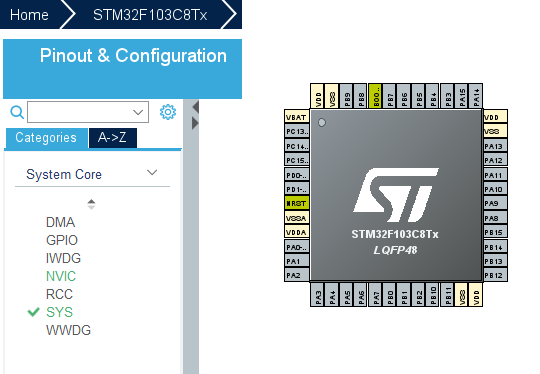
\includegraphics[width=\textwidth]{figure/4_1.png}
    \caption{GPIO configuration screen in STM Cube software}
    \label{fig:gpio-config}
\end{figure}

The GPIO driver provides many functions but the main ones used in this project:
\begin{enumerate}
    \item \textbf{HAL\_GPIO\_Init():} within the Main by default when performing the configuration and its purpose is to initialize the GPIO. A missing Init function would errors in case of the use of another GPIO function.
    \item \textbf{HAL\_delay():} responsible for delays between two commands and its argument is time measured in milliseconds.
    \item \textbf{HAL\_GPIO\_Write\_Pin():} used to output either HIGH or LOW for any pin already configured as output taking arguments of the port and the pin.
    \item \textbf{HAL\_GPIO\_Read\_Pin():} returns the value of a pin configured as input and takes the arguments as the port and the pin.
\end{enumerate}

\subsection{Timers}

An important peripheral acting as a clock, it’s indispensable to measure time and count values to give the needed output.In case of measuring the speed of the vehicle’s wheel the objective is to count the number of revolutions in a certain period, this is where the timer comes in.\\


Four timers are available each one has four channels which gives the possibility for 16 different timer dependant applications if the applications were chosen carefully to avoid conflict with the registers use. Each channel has a number of modes its uses will become apparent in the upcoming chapter. \\To activate the timer modifications have to be preformed on the RCC which is the processor’s clock. One of the advantages of using the HAL is that it generates settings for the RCC.\\

Going over the clock configuration in the program, which allows to set the clock, the desired frequency and whether to use internal or external clock as shown in  \ref{fig:timer-config}. Beware that the maximum for the STM is 72MHz and to reach it there would be a need for an external clock which is why the program gives you options to select from and values to change to reach the intended values as shown in figure \ref{fig:clock-config}.\\
\begin{figure}[h]
   \centering
    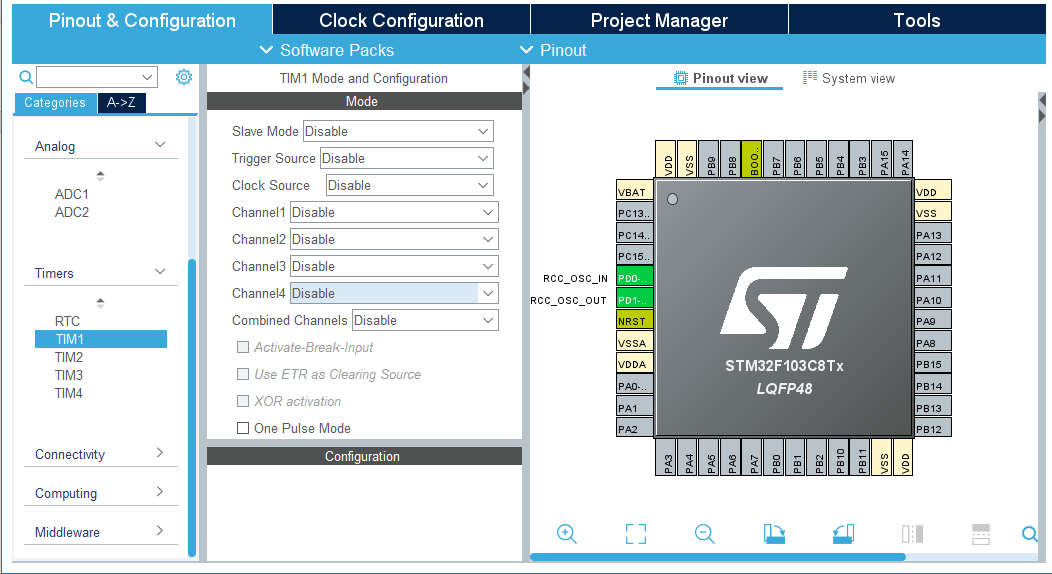
\includegraphics[width=.75\textwidth]{figure/4_2.png}
    \caption{Timer configuration screen in STM Cube software}
    \label{fig:timer-config}
\end{figure}
\begin{figure}[h]
   \centering
    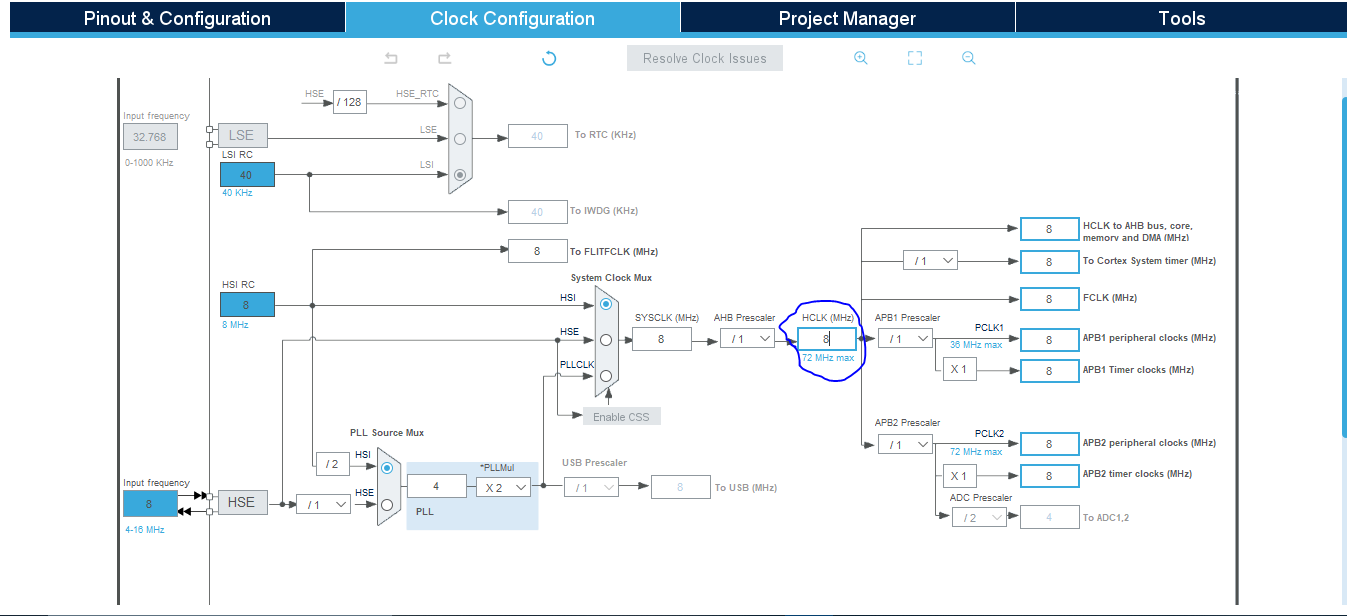
\includegraphics[width=.75\textwidth]{figure/4_3.png}
    \caption{Clock configuration screen in STM Cube software}
    \label{fig:clock-config}
\end{figure}

\clearpage

For the available functions provided by the HAL that are needed in the project:
\begin{enumerate}
    \item \textbf{MX\_TIMx\_Init():} written by default in the main to initiliaze the intended timers where the x is replaced by the number of the used timer.
    \item \textbf{HAL\_ROTARY\_Start():} used in the encoder mode which needs two channels per timer one internal and the second for the encoder.
\end{enumerate}

\subsection{Interrupts}

An important concept to understand is Nested Vector Interrupt Control (NVIC) which is available for some peripherals. If NVIC is enabled the HAL provides more functions for the intended peripheral such that the interrupt can be enabled with it. This is useful for the UART and the I2C.
The program also helps you organize each process that has its interrupt enabled by setting priority for each one. In case of two interrupts being activated at the same time the microcontroller will respond to the higher priority.\\
Some peripherals can be run in two possible methods, the first one called polling which activates the blocking mode. This method can cost more time however it is needed for certain tasks to be further explored in the upcoming chapter. The second method is the interrupt, in this case the process runs in the background meaning that it won’t be run unless the interrupt is activated which gives faster activation.\\
Additionally the STM also provides the Direct Memory Access Method but it wasn’t needed in the project.\\


\subsection{Universal asynchronous receiver-transmitter (UART)}

Universal asynchronous receiver-transmitter (UART) is indispensable part as it is the method of communication between the Raspberry Pi and the microcontroller.

\subsubsection{UART in the HAL library}
HAL library provides three methods can be used for UART communication
\begin{enumerate}
    \item Polling method: This method transmits/receives data in blocking mode and it will not allow any other operation to be implemented until the transmission/receive is done or time out occurred.
    \item Interrupt method: In this method, data transmission takes place in background or in non-blocking mode, When transmission is complete,\\ \textbf{HAL\_UART\_TxCpltCallback()} function is called, and the user can write inside this functions the instructions they need.
    \item DMA method: DMA works somewhat same as interrupt, meaning that data transfer is in non-blocking mode.\\

\end{enumerate}

In DMA, when half of the data get transferred, a half transfer get triggered and \textbf{HAL\_UART\_TxHalfCpltCallback()} function is called. The idea behind using DMA is when the second half of the data is being transferred, new data can be written in the first half section.

\subsubsection{Handle structure}

Handles contain information about related periphery and they are defined as global variables in the main file.\\

\emph{Handle structure consists of certain data types, some of them shown in the table below}

\begin{table}[h]
\def\arraystretch{1.5}
\centering
\begin{tabular}{| c | c |}
\hline
\cellcolor[HTML]{B4C6E7}Data   Type & \cellcolor[HTML]{B4C6E7}Value\\
Instance                            & USART1 or USART2\\
\hline
Baud rate                           & 9600 or 115200 \\
\hline
Status                              & Ready, Busy, and Error \\
\hline
Lock                                & Lock or unlock\\
\hline
Internal Status                     & TX or RX \\
\hline
*hdma tx pointer                    & DMA TX handler\\
\hline
*hdma rx pointer                    & DMA RX handler\\
\hline

\end{tabular}
\end{table}

i.e., when data is transmitted, first information is stored into the handler (how many bits to send, what is the baud rate, what is the status…etc.), after that they are sent to UART periphery. Not only the HAL function provides handler for USART1 and USART2, but also it provides handlers when the DMA method is used, and they are linked with UART handler together as shown below.\\

\subsubsection{HAL UART functions}

HAL functions are implemented to help the user to use the UART by the method they chose as well it provides system functions to initialize and set the UART, so the user does not need to initialize the registers and set the values for the UART.


\begin{enumerate}
    \item Initialization Functions:
    \begin{enumerate}
        \item \textbf{MX\_UART\_Init():}\\
        This function takes void arguement and returns void, it is called automatically in the code generated from STMCube, its functionalities are:
        \begin{itemize}
            \item Store UART parameters into initialize structure in UART handler
            \item Call \textbf{HAL\_UART\_Init()}
        \end{itemize}
        
        \item \textbf{HAL\_UART\_Init():}\\
        This function takes address of handler structure value and the returns void, it is called inside the \textbf{MX\_UART\_Init()}, its functionalities are:
        \begin{itemize}
            \item Store initialization structure (handler) into UART registers.
            \item Call \textbf{HAL\_UART\_MspInit()}
        \end{itemize}
        
        \item \textbf{HAL\_UART\_MspInit():}
        This function takes handler structure value and the returns void, its function is to initialize the GPIO parameters (pull up, speed, mode, pin state...etc.).\\
        
     
        \emph{Figure \ref{fig:init-flow-chart} summarizes initialization functions}
        
        \begin{figure}[h]
        \centering
        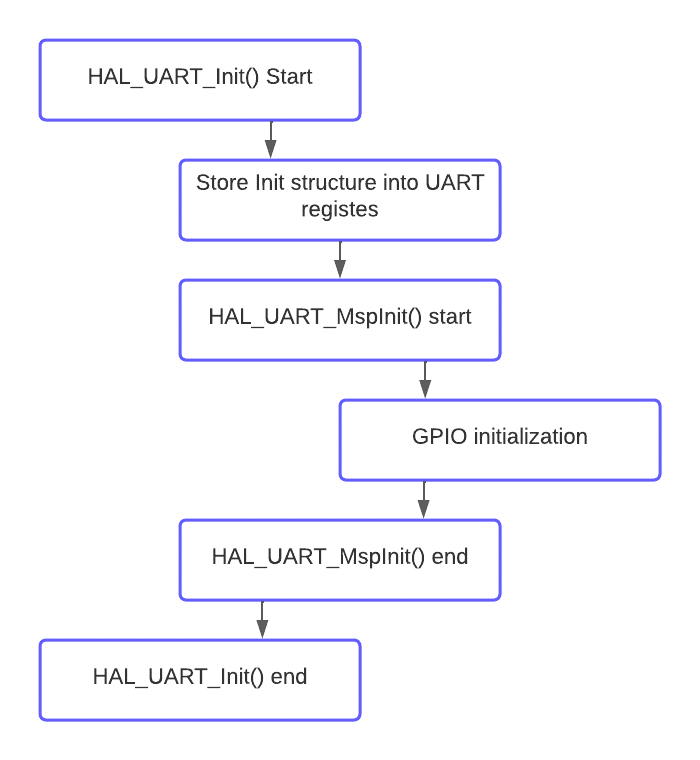
\includegraphics[width=.75\textwidth]{figure/4_4.png}
        \caption{Initialization functions flow chart}
        \label{fig:init-flow-chart}
    \end{figure}

    \clearpage
    \end{enumerate}
    \item User Functions:
    HAL library provides some functions for the three methods
    \begin{enumerate}
        \item Polling Method:
        HAL functions handle blocking polling processes, the functions that can be used are:
        \begin{itemize}
            \item \textbf{HAL\_UART\_Transmit():} This function takes four arguments; handler structure, buffer for data to be transmitted, size of buffer, and the time for transmitting and it returns HAL\_status prototype which it can be HAL\_OK, HAL\_BUSY, and HAL\_ERROR.
            \item \textbf{HAL\_UART\_Receive():} This function takes four arguments; handler structure, buffer for data to be received, size of buffer, and the time for receiving and it returns HAL\_status prototype which it can be HAL\_OK, HAL\_BUSY, and HAL\_ERROR.\\
            
            
        \end{itemize}
        \emph{Figure \ref{fig:user-func-flow-chart} shows a flow chart for which is inside the receive function (and the same in transmit function).}
            \begin{figure}[h]
            \centering
            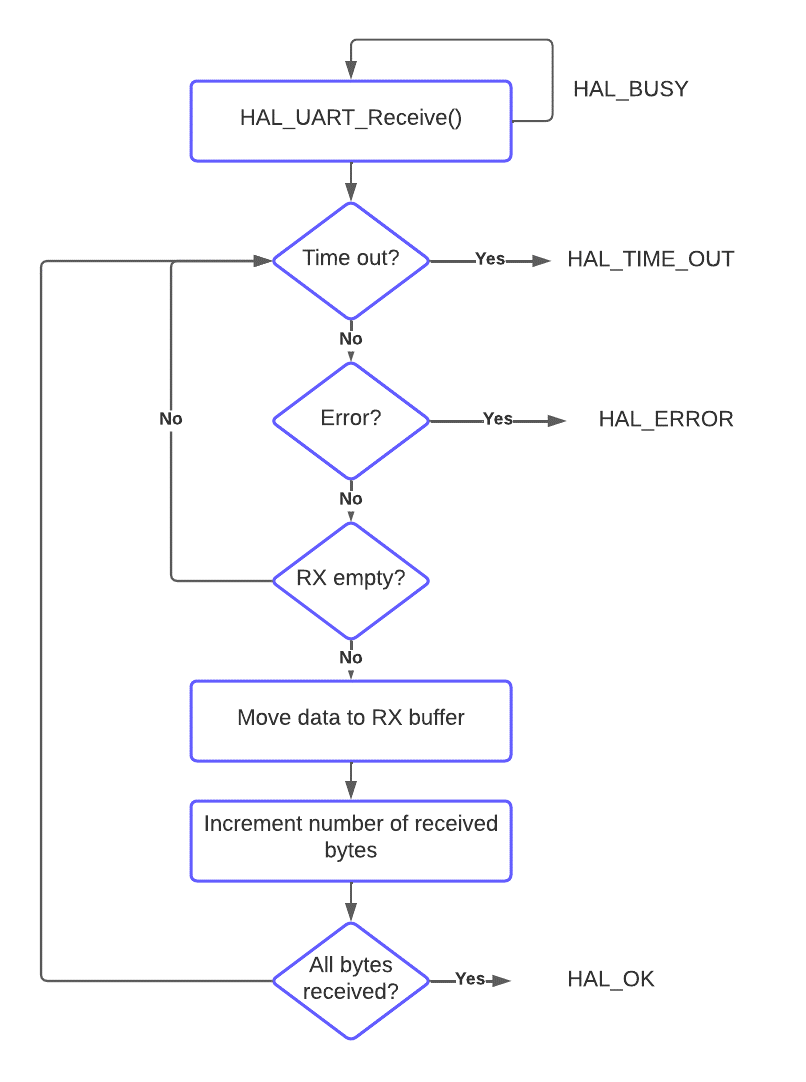
\includegraphics[width=.65\textwidth]{figure/4_5.png}
            \caption{User functions flow chart}
            \label{fig:user-func-flow-chart}
            \end{figure}

        \clearpage
        \item Interrupt Method:
        Interrupt method is used to solve the problem of blocking mode to make the process complete executing its processes and UART will be in the background (non-blocking mode).\\
        In this method, \textbf{HAL\_UART\_MspInit()} will call two new functions to handle the interrupt:
        
        \begin{itemize}
            \item \textbf{HAL\_NVIC\_SetPriority():} This function is to set the priority of the UART interrupt whether it has a low priority or high. NVIC stands to Nested Vector Interrupt Controller.
            \item \textbf{HAL\_NVIC\_EnableIRQ():} This function is to enable the handler of the interrupt. IRQ stands for interrupt request.
        \end{itemize}
        
        \emph{Also, HAL library provides other functions to be called when performs the receive/transmit functions:}
        \begin{itemize}
            \item \textbf{HAL\_UART\_Transmit\_IT():} “IT” stands for interrupt, this function takes three arguments; handler structure, buffer for data to be transmitted, and size of buffer, and it returns HAL\_status prototype which it can be HAL\_OK or HAL\_ERROR. 
            \item \textbf{HAL\_UART\_Receive\_IT():} This function takes three arguments; handler structure, buffer for data to be received, and size of buffer, and it returns \textbf{HAL\_status} prototype which it can be HAL\_OK or HAL\_ERROR.
            \item \textbf{HAL\_UART\_IRQHandler():} This function is to handle the interrupt request of the UART inside the system.
            \item \textbf{HAL\_UART\_RXcpltCallback():} “cpltCallback” stands for complete callback, this function is automatically called when \textbf{HAL\_UART\_Receive\_IT()} finishes its code, the user can write inside this function since it is used to be such as a flag for the ending of the receiving. 
            \item \textbf{HAL\_UART\_TXcpltCallback():} This function is automatically called when \textbf{HAL\_UART\_Transmit\_IT()} finishes its code, the user can write inside this function since it is used to be such as a flag for the ending of the transmission.

        \end{itemize}
        \clearpage
        \emph{Figure \ref{fig:interrupt-flow-chart} shows a flow chart for which is inside the interrupt receive function (and the same in transmit function).}\\
             \begin{figure}[h]
            \centering
            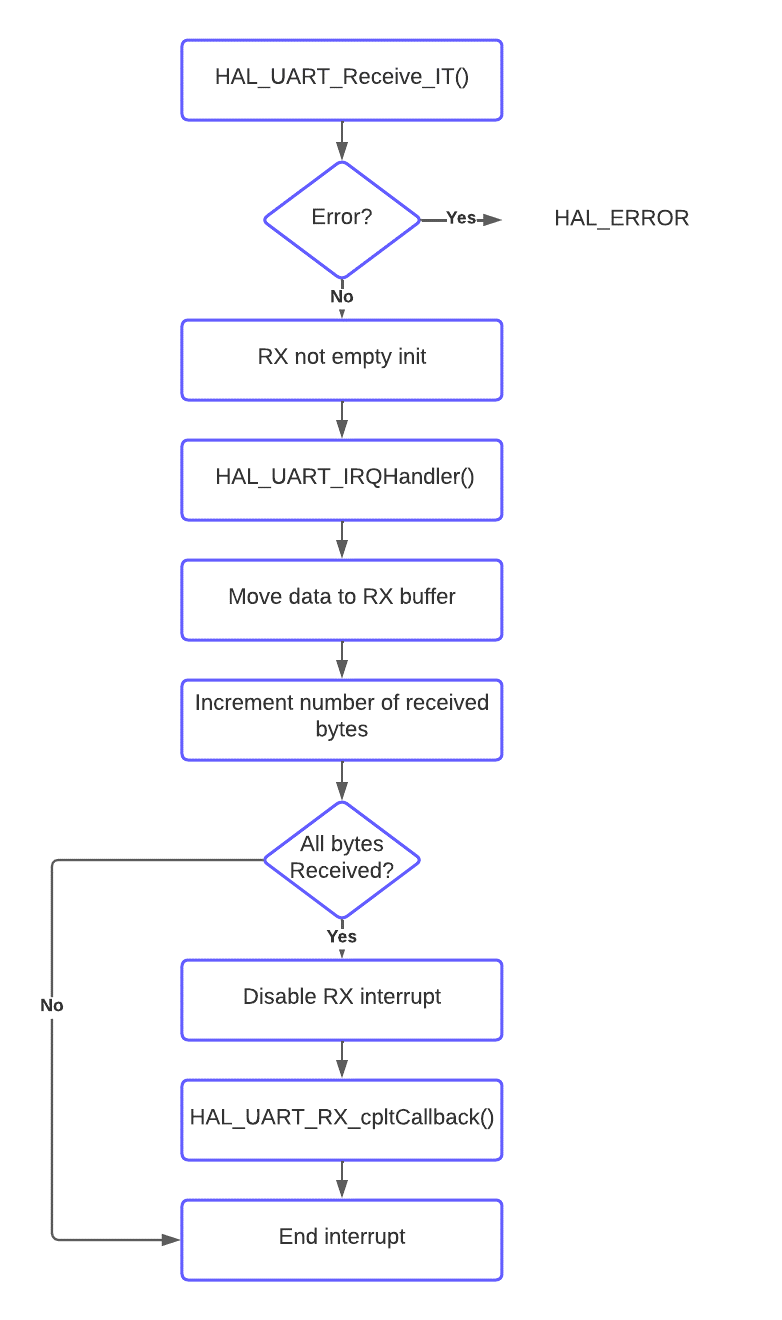
\includegraphics[width=.65\textwidth]{figure/4_6.png}
            \caption{Interrupt functions flow chart}
            \label{fig:interrupt-flow-chart}
            \end{figure}
       
    \end{enumerate}
\end{enumerate}

\subsection{Inter Integrated Circuit (I2C)}
 I2C is the method for communication between the micro-controller and some senors (IMU and Compass).\\
 
 Like UART, HAL library provides three methods that can be used for I2C communication
 \begin{enumerate}
     \item \textbf{I2C With Polling: }The first and the easiest way to do anything in embedded software is just to poll for the hardware
resource until it’s ready to move on to the next step in your program instructions. However, it’s

the least efficient way to do things and the CPU will end up wasting so much time in a “busy-
waiting” state.

It’s the same thing for both transmission and reception. You just wait until the current byte of data
to be transmitted so you can start the next one and so on.
     \item \textbf{I2C With Interrupts: } Enable the I2C interrupts can be done and have a signal when it’s done and ready for
servicing by CPU. Either for data that has been sent or received. Which saves a lot of time and
has been always the best way to handle events like that.
However, in some “Time Critical” applications everything is needed to be deterministic, in time,
as possible. And a major problem with interrupts is that it can’t be expected when it’d arrive or during
which task. That can potentially screw up the timing behavior of the system.
     \item \textbf{I2C With DMA: }
     To operate at its maximum speed, the I2C needs to be fed with the data for transmission and the
data received on the Rx buffer should be read to avoid overrun. To facilitate the transfers, the I2C
features a DMA capability implementing a simple request/acknowledge protocol.
 \end{enumerate}
 
 \subsubsection{I2C Configuration}
 
 Using STMCube, configuration is done by enabling an I2C from connectivity list as shown in figure \ref{fig:i2c-config}, and set the required parameters for masters and slaves. \\
 Note that I2C pins can be used in other modes instead of I2C, it can be used in Alert mode or bus two wire interface mode, but in the project the I2C mode is only needed.
 \newpage
 
 \begin{figure}
     \centering
     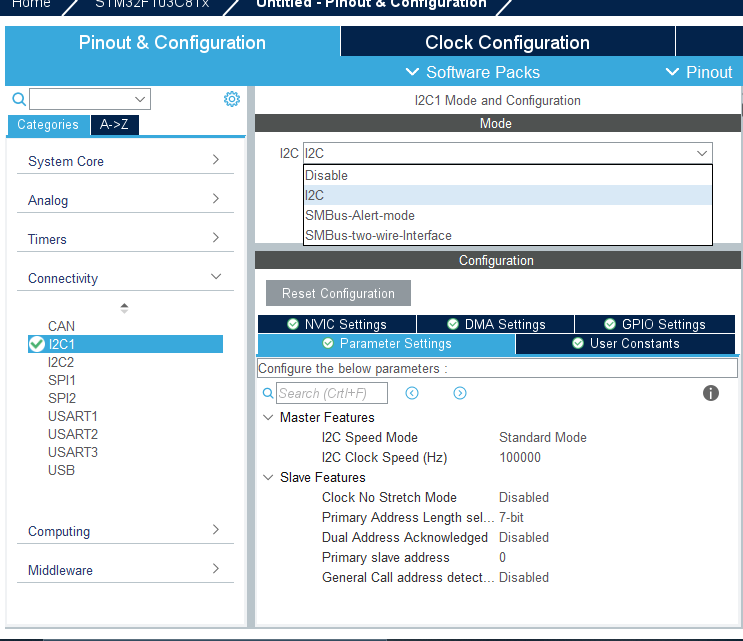
\includegraphics[width=.8\textwidth]{figure/4_7.png}
     \caption{I2C Configuration in STMCube}
     \label{fig:i2c-config}
 \end{figure}
 
 \subsubsection{I2C Functions}

For the available functions provided by the HAL that are needed in the project:

\begin{enumerate}
    \item \textbf{MX\textunderscore I2Cx\textunderscore Init()}: written by default in the main to initialize the intended I2C
where the x is replaced by the number of the used I2C.
    \item \textbf{HAL\textunderscore I2C\textunderscore Mem\textunderscore Write()}: This function is used to write the data on the I2C bus to send it to the connected slaves.
    \item \textbf{HAL\textunderscore I2C\textunderscore Mem\textunderscore Read()}: This function is used to read the data on the I2C bus that is sent by some slave.
\end{enumerate}